%==============================================================================
% ModelIR IEEE Paper - Supplementary Figures
% Choose from these to include in the main paper
%==============================================================================

\documentclass[conference]{IEEEtran}

\usepackage{amsmath}
\usepackage{graphicx}
\usepackage{tikz}
\usepackage{pgfplots}
\usepackage{booktabs}
\usepackage{subcaption}

\pgfplotsset{compat=1.17}
\usetikzlibrary{shapes.geometric, arrows.meta, positioning, fit, calc, patterns, decorations.pathreplacing}

\definecolor{parserblue}{RGB}{66,133,244}
\definecolor{irgreen}{RGB}{52,168,83}
\definecolor{writerorange}{RGB}{251,188,5}
\definecolor{verifyred}{RGB}{234,67,53}
\definecolor{lightblue}{RGB}{232,240,254}
\definecolor{lightgreen}{RGB}{232,245,233}
\definecolor{lightorange}{RGB}{255,248,225}
\definecolor{lightred}{RGB}{252,232,230}

\begin{document}

\title{Supplementary Figures for ModelIR Paper}
\maketitle

%==============================================================================
\section{Alternative Architecture Diagrams}
%==============================================================================

%------------------------------------------------------------------------------
% FIGURE OPTION A1: Vertical Architecture Diagram
%------------------------------------------------------------------------------
\begin{figure}[!t]
\centering
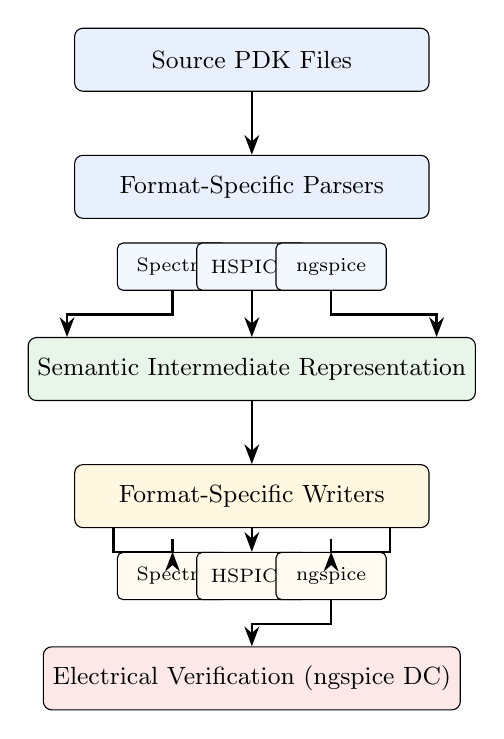
\begin{tikzpicture}[
    node distance=0.6cm,
    box/.style={rectangle, rounded corners=3pt, draw, minimum height=0.8cm, minimum width=4.5cm, font=\small, align=center},
    smallbox/.style={rectangle, rounded corners=2pt, draw, minimum height=0.6cm, minimum width=1.4cm, font=\scriptsize},
    arrow/.style={-{Stealth[length=2.5mm]}, thick}
]

% Input layer
\node[box, fill=lightblue] (input) {Source PDK Files};

% Parser layer
\node[box, fill=lightblue, below=0.8cm of input] (parsers) {Format-Specific Parsers};
\node[smallbox, fill=lightblue!50, below left=0.3cm and 0.3cm of parsers.south] (p1) {Spectre};
\node[smallbox, fill=lightblue!50, below=0.3cm of parsers.south] (p2) {HSPICE};
\node[smallbox, fill=lightblue!50, below right=0.3cm and 0.3cm of parsers.south] (p3) {ngspice};

% IR layer
\node[box, fill=lightgreen, below=1.5cm of parsers] (ir) {Semantic Intermediate Representation};

% Writer layer
\node[box, fill=lightorange, below=0.8cm of ir] (writers) {Format-Specific Writers};
\node[smallbox, fill=lightorange!50, below left=0.3cm and 0.3cm of writers.south] (w1) {Spectre};
\node[smallbox, fill=lightorange!50, below=0.3cm of writers.south] (w2) {HSPICE};
\node[smallbox, fill=lightorange!50, below right=0.3cm and 0.3cm of writers.south] (w3) {ngspice};

% Verification layer
\node[box, fill=lightred, below=1.5cm of writers] (verify) {Electrical Verification (ngspice DC)};

% Arrows
\draw[arrow] (input) -- (parsers);
\draw[arrow] (p1.south) -- ++(0,-0.3) -| ($(ir.north west)+(0.5,0)$);
\draw[arrow] (p2) -- (ir);
\draw[arrow] (p3.south) -- ++(0,-0.3) -| ($(ir.north east)+(-0.5,0)$);
\draw[arrow] (ir) -- (writers);
\draw[arrow] ($(writers.south west)+(0.5,0)$) -- ++(0,-0.3) -| (w1.north);
\draw[arrow] (writers) -- (w2);
\draw[arrow] ($(writers.south east)+(-0.5,0)$) -- ++(0,-0.3) -| (w3.north);
\draw[arrow] (w3.south) -- ++(0,-0.3) -| (verify);

\end{tikzpicture}
\caption{OPTION A1: Vertical architecture diagram showing the complete translation pipeline with format-specific parsers converging to a unified IR.}
\label{fig:arch_vertical}
\end{figure}

%------------------------------------------------------------------------------
% FIGURE OPTION A2: Compact Horizontal Pipeline
%------------------------------------------------------------------------------
\begin{figure}[!t]
\centering
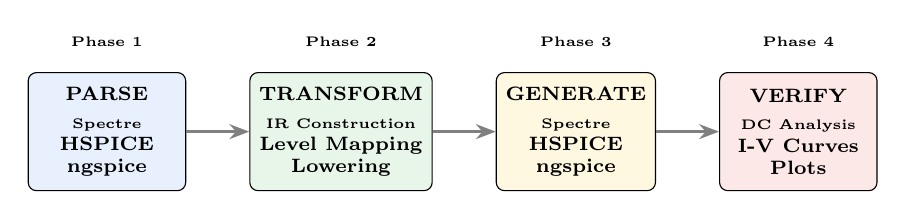
\begin{tikzpicture}[
    node distance=0.4cm,
    phase/.style={rectangle, rounded corners=3pt, draw, fill=#1, minimum height=1.5cm, minimum width=2cm, font=\scriptsize\bfseries, align=center},
    arrow/.style={-{Stealth[length=2.5mm]}, very thick, gray}
]

\node[phase=lightblue] (parse) {PARSE\\[2pt]\tiny Spectre\\HSPICE\\ngspice};
\node[phase=lightgreen, right=0.8cm of parse] (transform) {TRANSFORM\\[2pt]\tiny IR Construction\\Level Mapping\\Lowering};
\node[phase=lightorange, right=0.8cm of transform] (generate) {GENERATE\\[2pt]\tiny Spectre\\HSPICE\\ngspice};
\node[phase=lightred, right=0.8cm of generate] (verify) {VERIFY\\[2pt]\tiny DC Analysis\\I-V Curves\\Plots};

\draw[arrow] (parse) -- (transform);
\draw[arrow] (transform) -- (generate);
\draw[arrow] (generate) -- (verify);

% Phase labels
\node[above=0.2cm of parse, font=\tiny\bfseries] {Phase 1};
\node[above=0.2cm of transform, font=\tiny\bfseries] {Phase 2};
\node[above=0.2cm of generate, font=\tiny\bfseries] {Phase 3};
\node[above=0.2cm of verify, font=\tiny\bfseries] {Phase 4};

\end{tikzpicture}
\caption{OPTION A2: Compact horizontal pipeline showing the four main phases with their key operations.}
\label{fig:arch_compact}
\end{figure}

%------------------------------------------------------------------------------
% FIGURE OPTION A3: Detailed Component Diagram
%------------------------------------------------------------------------------
\begin{figure}[!t]
\centering
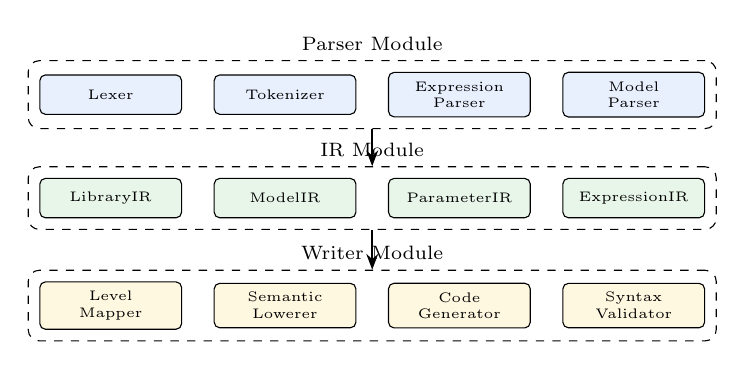
\begin{tikzpicture}[
    node distance=0.3cm,
    component/.style={rectangle, draw, rounded corners=2pt, minimum height=0.5cm, minimum width=1.8cm, font=\tiny, align=center},
    module/.style={rectangle, draw, dashed, rounded corners=4pt, inner sep=4pt},
    arrow/.style={-{Stealth[length=2mm]}, thick}
]

% Parser Module
\node[component, fill=lightblue] (lexer) {Lexer};
\node[component, fill=lightblue, right=0.4cm of lexer] (tokenizer) {Tokenizer};
\node[component, fill=lightblue, right=0.4cm of tokenizer] (exprparse) {Expression\\Parser};
\node[component, fill=lightblue, right=0.4cm of exprparse] (modelparse) {Model\\Parser};
\node[module, fit=(lexer)(tokenizer)(exprparse)(modelparse), label={[font=\scriptsize]above:Parser Module}] (pmodule) {};

% IR Module
\node[component, fill=lightgreen, below=0.8cm of lexer] (libir) {LibraryIR};
\node[component, fill=lightgreen, right=0.4cm of libir] (modelir) {ModelIR};
\node[component, fill=lightgreen, right=0.4cm of modelir] (paramair) {ParameterIR};
\node[component, fill=lightgreen, right=0.4cm of paramair] (exprir) {ExpressionIR};
\node[module, fit=(libir)(modelir)(paramair)(exprir), label={[font=\scriptsize]above:IR Module}] (irmodule) {};

% Writer Module
\node[component, fill=lightorange, below=0.8cm of libir] (levmap) {Level\\Mapper};
\node[component, fill=lightorange, right=0.4cm of levmap] (lower) {Semantic\\Lowerer};
\node[component, fill=lightorange, right=0.4cm of lower] (codegen) {Code\\Generator};
\node[component, fill=lightorange, right=0.4cm of codegen] (syntax) {Syntax\\Validator};
\node[module, fit=(levmap)(lower)(codegen)(syntax), label={[font=\scriptsize]above:Writer Module}] (wmodule) {};

% Arrows between modules
\draw[arrow] (pmodule.south) -- (irmodule.north);
\draw[arrow] (irmodule.south) -- (wmodule.north);

\end{tikzpicture}
\caption{OPTION A3: Detailed component diagram showing internal structure of each module.}
\label{fig:arch_detailed}
\end{figure}

%==============================================================================
\section{Alternative IR Diagrams}
%==============================================================================

%------------------------------------------------------------------------------
% FIGURE OPTION B1: IR as Tree Structure
%------------------------------------------------------------------------------
\begin{figure}[!t]
\centering
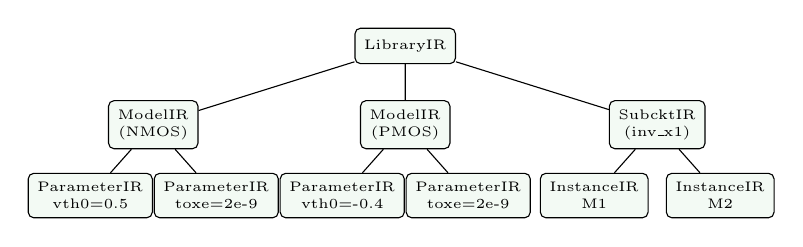
\begin{tikzpicture}[
    level 1/.style={sibling distance=3.2cm, level distance=1cm},
    level 2/.style={sibling distance=1.6cm, level distance=0.9cm},
    level 3/.style={sibling distance=1cm, level distance=0.8cm},
    every node/.style={rectangle, rounded corners=2pt, draw, fill=lightgreen!50, font=\tiny, minimum height=0.45cm, minimum width=0.8cm, align=center}
]

\node {LibraryIR}
    child { node {ModelIR\\(NMOS)}
        child { node {ParameterIR\\vth0=0.5} }
        child { node {ParameterIR\\toxe=2e-9} }
    }
    child { node {ModelIR\\(PMOS)}
        child { node {ParameterIR\\vth0=-0.4} }
        child { node {ParameterIR\\toxe=2e-9} }
    }
    child { node {SubcktIR\\(inv\_x1)}
        child { node {InstanceIR\\M1} }
        child { node {InstanceIR\\M2} }
    };

\end{tikzpicture}
\caption{OPTION B1: IR as a tree structure showing the hierarchical organization of a model library with NMOS, PMOS models and an inverter subcircuit.}
\label{fig:ir_tree}
\end{figure}

%------------------------------------------------------------------------------
% FIGURE OPTION B2: IR with Semantic Annotations
%------------------------------------------------------------------------------
\begin{figure}[!t]
\centering
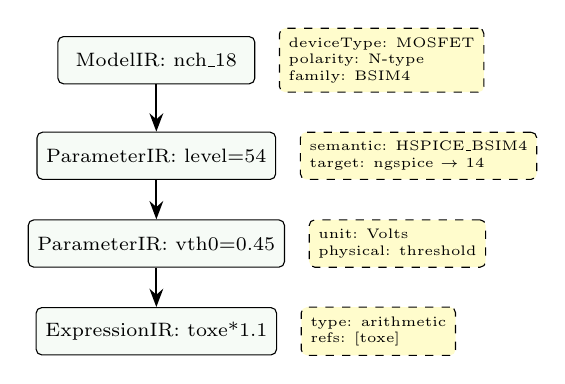
\begin{tikzpicture}[
    node distance=0.3cm,
    irbox/.style={rectangle, draw, rounded corners=2pt, fill=lightgreen!40, minimum height=0.6cm, minimum width=2.5cm, font=\scriptsize},
    annot/.style={rectangle, draw, dashed, rounded corners=2pt, fill=yellow!20, minimum height=0.4cm, font=\tiny, align=left}
]

\node[irbox] (model) {ModelIR: nch\_18};
\node[annot, right=0.3cm of model] (a1) {deviceType: MOSFET\\polarity: N-type\\family: BSIM4};

\node[irbox, below=0.6cm of model] (param1) {ParameterIR: level=54};
\node[annot, right=0.3cm of param1] (a2) {semantic: HSPICE\_BSIM4\\target: ngspice $\rightarrow$ 14};

\node[irbox, below=0.5cm of param1] (param2) {ParameterIR: vth0=0.45};
\node[annot, right=0.3cm of param2] (a3) {unit: Volts\\physical: threshold};

\node[irbox, below=0.5cm of param2] (expr) {ExpressionIR: toxe*1.1};
\node[annot, right=0.3cm of expr] (a4) {type: arithmetic\\refs: [toxe]};

\draw[-{Stealth}, thick] (model) -- (param1);
\draw[-{Stealth}, thick] (param1) -- (param2);
\draw[-{Stealth}, thick] (param2) -- (expr);

\end{tikzpicture}
\caption{OPTION B2: IR nodes with semantic annotations showing how device physics metadata is attached to each IR element.}
\label{fig:ir_annotated}
\end{figure}

%==============================================================================
\section{Alternative Lowering Diagrams}
%==============================================================================

%------------------------------------------------------------------------------
% FIGURE OPTION C1: Multi-Example Lowering
%------------------------------------------------------------------------------
\begin{figure}[!t]
\centering
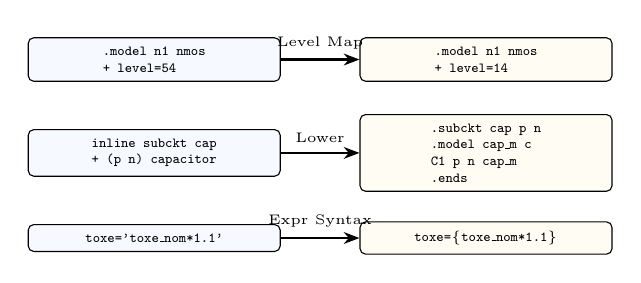
\begin{tikzpicture}[
    node distance=0.3cm,
    srcbox/.style={rectangle, draw, rounded corners=2pt, fill=lightblue!40, minimum width=3.2cm, font=\tiny\ttfamily, align=left},
    tgtbox/.style={rectangle, draw, rounded corners=2pt, fill=lightorange!40, minimum width=3.2cm, font=\tiny\ttfamily, align=left},
    arrow/.style={-{Stealth[length=2mm]}, thick}
]

% Example 1: Level mapping
\node[srcbox] (src1) {.model n1 nmos\\+ level=54};
\node[tgtbox, right=1cm of src1] (tgt1) {.model n1 nmos\\+ level=14};
\draw[arrow] (src1) -- node[above, font=\tiny] {Level Map} (tgt1);

% Example 2: Inline subckt
\node[srcbox, below=0.6cm of src1] (src2) {inline subckt cap\\+ (p n) capacitor};
\node[tgtbox, right=1cm of src2] (tgt2) {.subckt cap p n\\.model cap\_m c\\C1 p n cap\_m\\.ends};
\draw[arrow] (src2) -- node[above, font=\tiny] {Lower} (tgt2);

% Example 3: Expression
\node[srcbox, below=0.6cm of src2] (src3) {toxe='toxe\_nom*1.1'};
\node[tgtbox, right=1cm of src3] (tgt3) {toxe=\{toxe\_nom*1.1\}};
\draw[arrow] (src3) -- node[above, font=\tiny] {Expr Syntax} (tgt3);

\end{tikzpicture}
\caption{OPTION C1: Multiple lowering examples showing level mapping, inline subcircuit expansion, and expression syntax conversion.}
\label{fig:lowering_multi}
\end{figure}

%==============================================================================
\section{Alternative Performance Charts}
%==============================================================================

%------------------------------------------------------------------------------
% FIGURE OPTION D1: Per-PDK Success Rate Bar Chart
%------------------------------------------------------------------------------
\begin{figure}[!t]
\centering
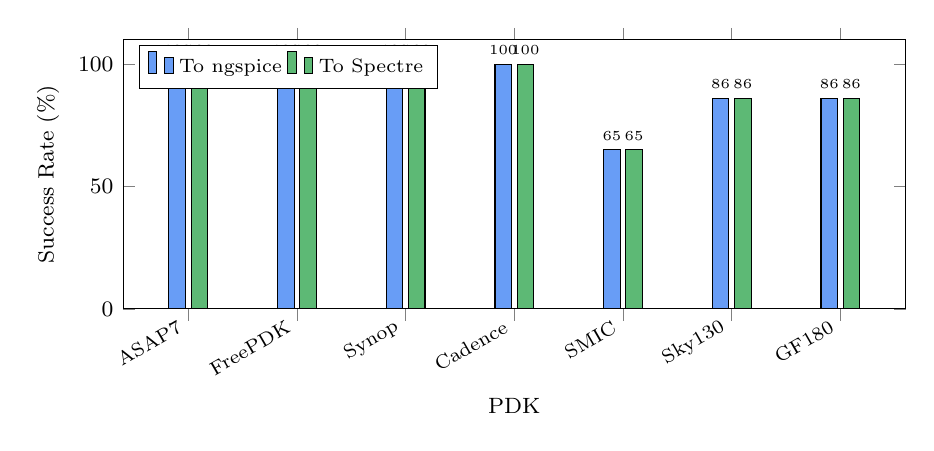
\begin{tikzpicture}
\begin{axis}[
    ybar,
    width=0.95\columnwidth,
    height=5cm,
    bar width=6pt,
    xlabel={PDK},
    ylabel={Success Rate (\%)},
    xlabel style={font=\footnotesize},
    ylabel style={font=\footnotesize},
    symbolic x coords={ASAP7, FreePDK, Synop, Cadence, SMIC, Sky130, GF180},
    xtick=data,
    xticklabel style={font=\scriptsize, rotate=30, anchor=east},
    yticklabel style={font=\footnotesize},
    ymin=0, ymax=110,
    nodes near coords,
    nodes near coords style={font=\tiny},
    enlarge x limits=0.1,
    legend style={at={(0.02,0.98)}, anchor=north west, font=\scriptsize},
    legend columns=2,
]
\addplot[fill=parserblue!80] coordinates {
    (ASAP7, 100) (FreePDK, 100) (Synop, 100) (Cadence, 100) (SMIC, 65) (Sky130, 86) (GF180, 86)
};
\addlegendentry{To ngspice}
\addplot[fill=irgreen!80] coordinates {
    (ASAP7, 100) (FreePDK, 100) (Synop, 100) (Cadence, 100) (SMIC, 65) (Sky130, 86) (GF180, 86)
};
\addlegendentry{To Spectre}
\end{axis}
\end{tikzpicture}
\caption{OPTION D1: Translation success rate by PDK family, showing both ngspice and Spectre target formats.}
\label{fig:pdk_success}
\end{figure}

%------------------------------------------------------------------------------
% FIGURE OPTION D2: Stacked Model Distribution
%------------------------------------------------------------------------------
\begin{figure}[!t]
\centering
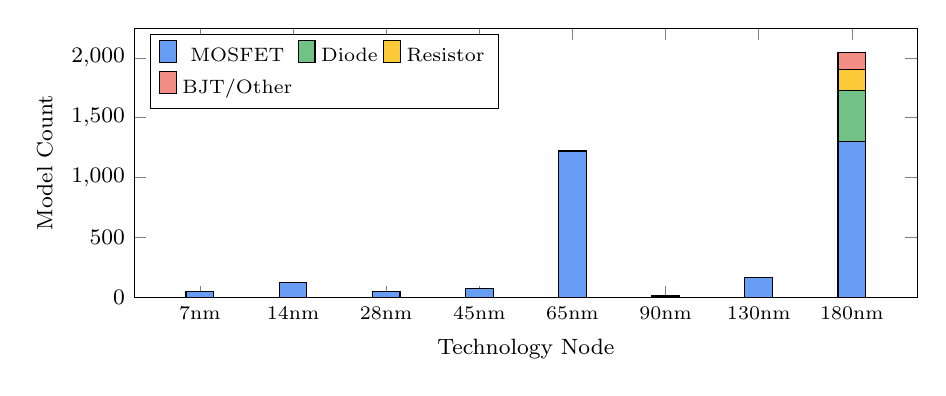
\begin{tikzpicture}
\begin{axis}[
    ybar stacked,
    width=0.95\columnwidth,
    height=5cm,
    bar width=10pt,
    xlabel={Technology Node},
    ylabel={Model Count},
    xlabel style={font=\footnotesize},
    ylabel style={font=\footnotesize},
    symbolic x coords={7nm, 14nm, 28nm, 45nm, 65nm, 90nm, 130nm, 180nm},
    xtick=data,
    xticklabel style={font=\scriptsize},
    yticklabel style={font=\footnotesize},
    ymin=0,
    legend style={at={(0.02,0.98)}, anchor=north west, font=\scriptsize, legend columns=3},
    enlarge x limits=0.1,
]
\addplot[fill=parserblue!80] coordinates {(7nm, 48) (14nm, 128) (28nm, 48) (45nm, 76) (65nm, 1222) (90nm, 12) (130nm, 168) (180nm, 1305)};
\addlegendentry{MOSFET}
\addplot[fill=irgreen!70] coordinates {(7nm, 0) (14nm, 0) (28nm, 0) (45nm, 0) (65nm, 0) (90nm, 0) (130nm, 0) (180nm, 420)};
\addlegendentry{Diode}
\addplot[fill=writerorange!80] coordinates {(7nm, 0) (14nm, 0) (28nm, 0) (45nm, 0) (65nm, 0) (90nm, 0) (130nm, 0) (180nm, 180)};
\addlegendentry{Resistor}
\addplot[fill=verifyred!60] coordinates {(7nm, 0) (14nm, 0) (28nm, 0) (45nm, 0) (65nm, 0) (90nm, 0) (130nm, 0) (180nm, 138)};
\addlegendentry{BJT/Other}
\end{axis}
\end{tikzpicture}
\caption{OPTION D2: Model count by technology node with device type breakdown. 180nm and 65nm nodes dominate due to mature PDK availability.}
\label{fig:node_dist}
\end{figure}

%------------------------------------------------------------------------------
% FIGURE OPTION D3: Pie Chart Device Distribution
%------------------------------------------------------------------------------
\begin{figure}[!t]
\centering
\begin{tikzpicture}
\pie[
    radius=2.2,
    text=legend,
    color={parserblue!80, irgreen!70, writerorange!80, verifyred!60, gray!50},
    explode={0.1, 0, 0, 0, 0},
    font=\scriptsize
]{
    58.6/MOSFET (2654),
    19.7/Diode (892),
    11.8/Resistor (534),
    6.9/Capacitor (312),
    3.0/BJT (138)
}
\end{tikzpicture}
\caption{OPTION D3: Pie chart showing device type distribution across all translated models.}
\label{fig:device_pie}
\end{figure}

%------------------------------------------------------------------------------
% FIGURE OPTION D4: Translation Time Histogram
%------------------------------------------------------------------------------
\begin{figure}[!t]
\centering
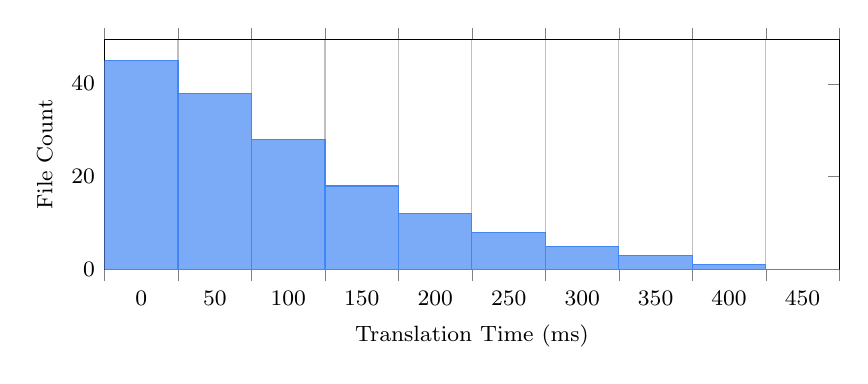
\begin{tikzpicture}
\begin{axis}[
    ybar interval,
    width=0.9\columnwidth,
    height=4.5cm,
    xlabel={Translation Time (ms)},
    ylabel={File Count},
    xlabel style={font=\footnotesize},
    ylabel style={font=\footnotesize},
    xticklabel style={font=\footnotesize},
    yticklabel style={font=\footnotesize},
    xmin=0, xmax=500,
    ymin=0,
]
\addplot[fill=parserblue!70, draw=parserblue] coordinates {
    (0, 45) (50, 38) (100, 28) (150, 18) (200, 12) (250, 8) (300, 5) (350, 3) (400, 1) (450, 0) (500, 0)
};
\end{axis}
\end{tikzpicture}
\caption{OPTION D4: Histogram of per-file translation times. Most files complete in under 100ms.}
\label{fig:time_hist}
\end{figure}

%==============================================================================
\section{Alternative I-V Curve Presentations}
%==============================================================================

%------------------------------------------------------------------------------
% FIGURE OPTION E1: 4-Panel I-V Characteristics
%------------------------------------------------------------------------------
\begin{figure*}[!t]
\centering
\begin{subfigure}[b]{0.24\textwidth}
\centering
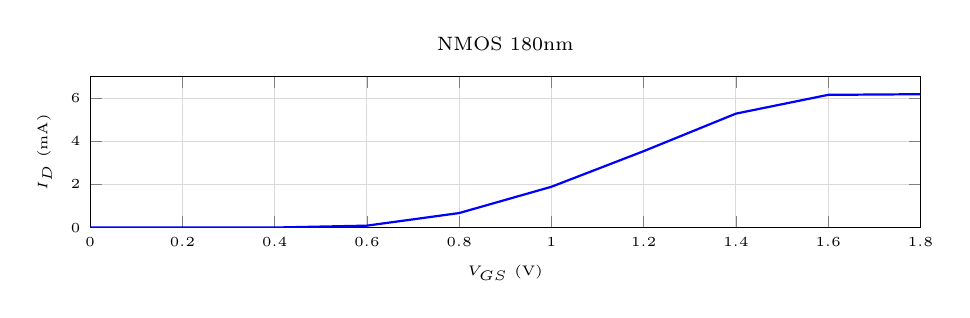
\begin{tikzpicture}
\begin{axis}[
    width=\textwidth,
    height=3.5cm,
    xlabel={$V_{GS}$ (V)},
    ylabel={$I_D$ (mA)},
    xlabel style={font=\tiny},
    ylabel style={font=\tiny},
    xticklabel style={font=\tiny},
    yticklabel style={font=\tiny},
    xmin=0, xmax=1.8, ymin=0, ymax=7,
    grid=major, grid style={gray!30},
    title={\scriptsize NMOS 180nm},
    title style={font=\scriptsize},
]
\addplot[blue, thick] coordinates {
    (0,0) (0.4,0.001) (0.6,0.089) (0.8,0.672) (1.0,1.89) (1.2,3.54) (1.4,5.28) (1.6,6.15) (1.8,6.18)
};
\end{axis}
\end{tikzpicture}
\caption{$I_D$-$V_{GS}$ transfer}
\end{subfigure}
\hfill
\begin{subfigure}[b]{0.24\textwidth}
\centering
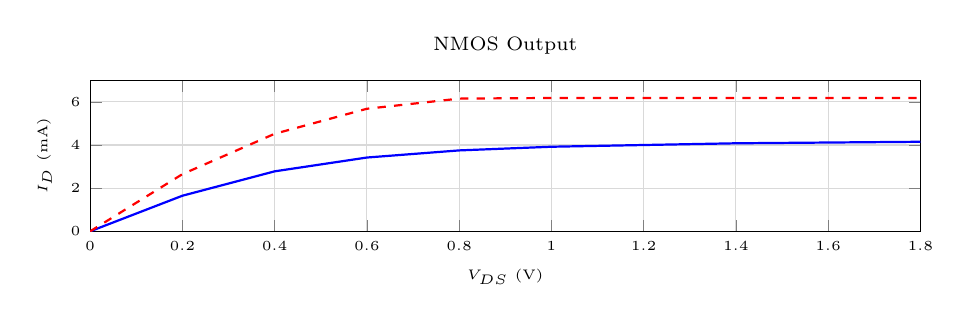
\begin{tikzpicture}
\begin{axis}[
    width=\textwidth,
    height=3.5cm,
    xlabel={$V_{DS}$ (V)},
    ylabel={$I_D$ (mA)},
    xlabel style={font=\tiny},
    ylabel style={font=\tiny},
    xticklabel style={font=\tiny},
    yticklabel style={font=\tiny},
    xmin=0, xmax=1.8, ymin=0, ymax=7,
    grid=major, grid style={gray!30},
    title={\scriptsize NMOS Output},
    title style={font=\scriptsize},
]
\addplot[blue, thick] coordinates {(0,0) (0.2,1.65) (0.4,2.78) (0.6,3.42) (0.8,3.75) (1.0,3.92) (1.4,4.08) (1.8,4.15)};
\addplot[red, thick, dashed] coordinates {(0,0) (0.2,2.65) (0.4,4.52) (0.6,5.68) (0.8,6.15) (1.0,6.18) (1.8,6.18)};
\end{axis}
\end{tikzpicture}
\caption{$I_D$-$V_{DS}$ output}
\end{subfigure}
\hfill
\begin{subfigure}[b]{0.24\textwidth}
\centering
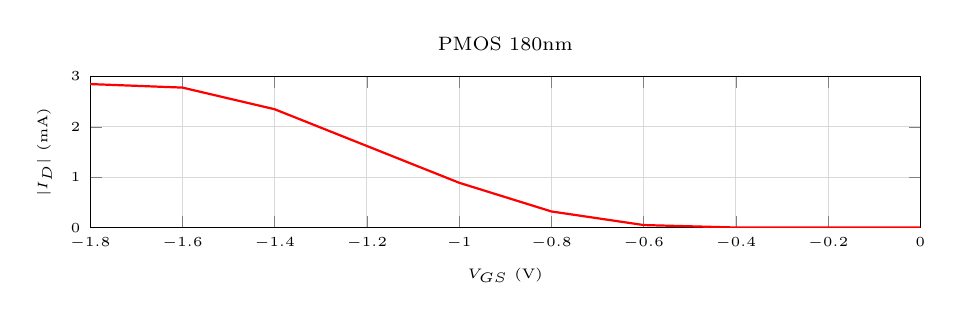
\begin{tikzpicture}
\begin{axis}[
    width=\textwidth,
    height=3.5cm,
    xlabel={$V_{GS}$ (V)},
    ylabel={$|I_D|$ (mA)},
    xlabel style={font=\tiny},
    ylabel style={font=\tiny},
    xticklabel style={font=\tiny},
    yticklabel style={font=\tiny},
    xmin=-1.8, xmax=0, ymin=0, ymax=3,
    grid=major, grid style={gray!30},
    title={\scriptsize PMOS 180nm},
    title style={font=\scriptsize},
]
\addplot[red, thick] coordinates {
    (0,0) (-0.4,0.001) (-0.6,0.05) (-0.8,0.32) (-1.0,0.89) (-1.2,1.62) (-1.4,2.35) (-1.6,2.78) (-1.8,2.85)
};
\end{axis}
\end{tikzpicture}
\caption{PMOS transfer}
\end{subfigure}
\hfill
\begin{subfigure}[b]{0.24\textwidth}
\centering
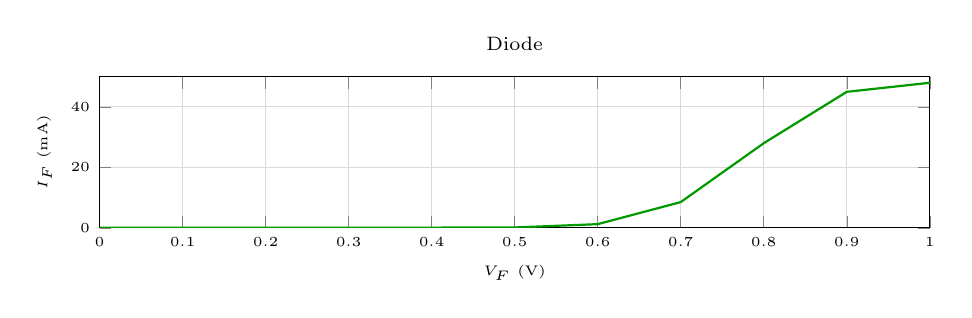
\begin{tikzpicture}
\begin{axis}[
    width=\textwidth,
    height=3.5cm,
    xlabel={$V_F$ (V)},
    ylabel={$I_F$ (mA)},
    xlabel style={font=\tiny},
    ylabel style={font=\tiny},
    xticklabel style={font=\tiny},
    yticklabel style={font=\tiny},
    xmin=0, xmax=1, ymin=0, ymax=50,
    grid=major, grid style={gray!30},
    title={\scriptsize Diode},
    title style={font=\scriptsize},
]
\addplot[green!60!black, thick] coordinates {
    (0,0) (0.3,0.001) (0.5,0.1) (0.6,1.2) (0.7,8.5) (0.8,28) (0.9,45) (1.0,48)
};
\end{axis}
\end{tikzpicture}
\caption{Diode forward}
\end{subfigure}
\caption{OPTION E1: Four-panel I-V characteristics showing NMOS transfer/output, PMOS transfer, and diode forward characteristics from translated 180nm models.}
\label{fig:iv_4panel}
\end{figure*}

%------------------------------------------------------------------------------
% FIGURE OPTION E2: Log-Scale Subthreshold
%------------------------------------------------------------------------------
\begin{figure}[!t]
\centering
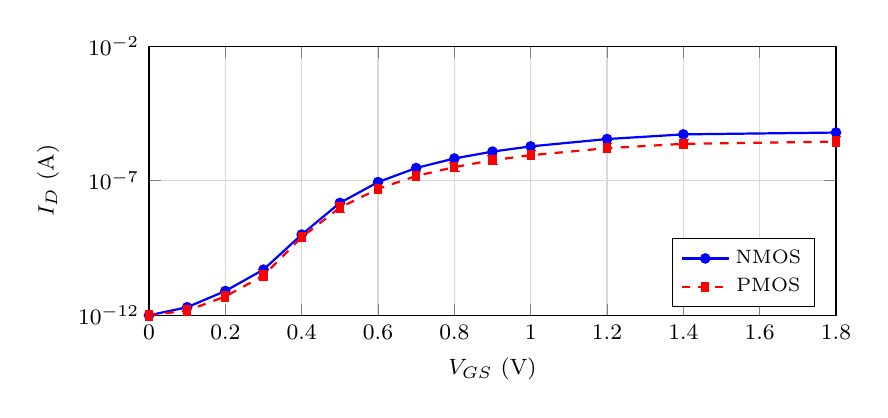
\begin{tikzpicture}
\begin{semilogyaxis}[
    width=0.85\columnwidth,
    height=5cm,
    xlabel={$V_{GS}$ (V)},
    ylabel={$I_D$ (A)},
    xlabel style={font=\footnotesize},
    ylabel style={font=\footnotesize},
    xticklabel style={font=\footnotesize},
    yticklabel style={font=\footnotesize},
    xmin=0, xmax=1.8,
    ymin=1e-12, ymax=1e-2,
    grid=major, grid style={gray!30},
    legend pos=south east,
    legend style={font=\scriptsize},
]
\addplot[blue, thick, mark=*, mark size=1.5pt] coordinates {
    (0.0, 1e-12) (0.1, 2e-12) (0.2, 8e-12) (0.3, 5e-11) (0.4, 1e-9)
    (0.5, 1.5e-8) (0.6, 8.9e-8) (0.7, 2.98e-7) (0.8, 6.72e-7)
    (0.9, 1.21e-6) (1.0, 1.89e-6) (1.2, 3.54e-6) (1.4, 5.28e-6) (1.8, 6.18e-6)
};
\addlegendentry{NMOS}
\addplot[red, thick, dashed, mark=square*, mark size=1.5pt] coordinates {
    (0.0, 1e-12) (0.1, 1.5e-12) (0.2, 5e-12) (0.3, 3e-11) (0.4, 8e-10)
    (0.5, 1e-8) (0.6, 5e-8) (0.7, 1.5e-7) (0.8, 3.2e-7)
    (0.9, 5.8e-7) (1.0, 8.9e-7) (1.2, 1.62e-6) (1.4, 2.35e-6) (1.8, 2.85e-6)
};
\addlegendentry{PMOS}
\end{semilogyaxis}
\end{tikzpicture}
\caption{OPTION E2: Semi-log plot of drain current showing subthreshold characteristics and on/off ratio for both NMOS and PMOS devices.}
\label{fig:iv_log}
\end{figure}

%==============================================================================
\section{Alternative Verification Diagrams}
%==============================================================================

%------------------------------------------------------------------------------
% FIGURE OPTION F1: Verification Results Summary
%------------------------------------------------------------------------------
\begin{figure}[!t]
\centering
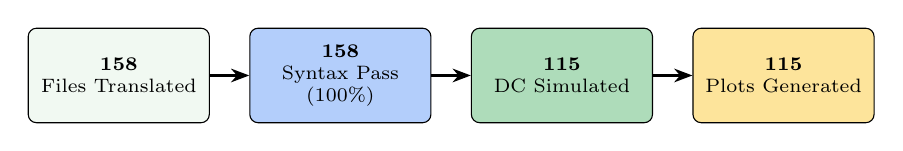
\begin{tikzpicture}[
    node distance=0.4cm,
    statbox/.style={rectangle, draw, rounded corners=3pt, minimum height=1.2cm, minimum width=2.3cm, font=\scriptsize, align=center},
]

\node[statbox, fill=lightgreen!60] (total) {\textbf{158}\\Files Translated};
\node[statbox, fill=parserblue!40, right=0.5cm of total] (syntax) {\textbf{158}\\Syntax Pass\\(100\%)};
\node[statbox, fill=irgreen!40, right=0.5cm of syntax] (sim) {\textbf{115}\\DC Simulated};
\node[statbox, fill=writerorange!40, right=0.5cm of sim] (plots) {\textbf{115}\\Plots Generated};

\draw[-{Stealth}, thick] (total) -- (syntax);
\draw[-{Stealth}, thick] (syntax) -- (sim);
\draw[-{Stealth}, thick] (sim) -- (plots);

\end{tikzpicture}
\caption{OPTION F1: Verification results flow showing 100\% syntax pass rate and 115 DC simulations with plot generation.}
\label{fig:verify_flow}
\end{figure}

%------------------------------------------------------------------------------
% FIGURE OPTION F2: Verification by Device Type
%------------------------------------------------------------------------------
\begin{figure}[!t]
\centering
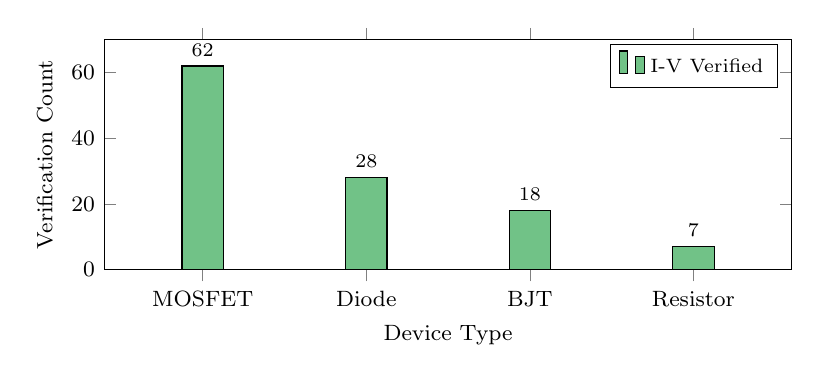
\begin{tikzpicture}
\begin{axis}[
    ybar,
    width=0.85\columnwidth,
    height=4.5cm,
    bar width=15pt,
    xlabel={Device Type},
    ylabel={Verification Count},
    xlabel style={font=\footnotesize},
    ylabel style={font=\footnotesize},
    symbolic x coords={MOSFET, Diode, BJT, Resistor},
    xtick=data,
    xticklabel style={font=\footnotesize},
    yticklabel style={font=\footnotesize},
    nodes near coords,
    nodes near coords style={font=\scriptsize},
    ymin=0, ymax=70,
    legend style={at={(0.98,0.98)}, anchor=north east, font=\scriptsize},
    enlarge x limits=0.2,
]
\addplot[fill=irgreen!70] coordinates {(MOSFET, 62) (Diode, 28) (BJT, 18) (Resistor, 7)};
\addlegendentry{I-V Verified}
\end{axis}
\end{tikzpicture}
\caption{OPTION F2: Number of models with I-V verification by device type.}
\label{fig:verify_device}
\end{figure}

%==============================================================================
\section{Include Resolution Diagram}
%==============================================================================

%------------------------------------------------------------------------------
% FIGURE OPTION G1: Include Resolution Workflow
%------------------------------------------------------------------------------
\begin{figure}[!t]
\centering
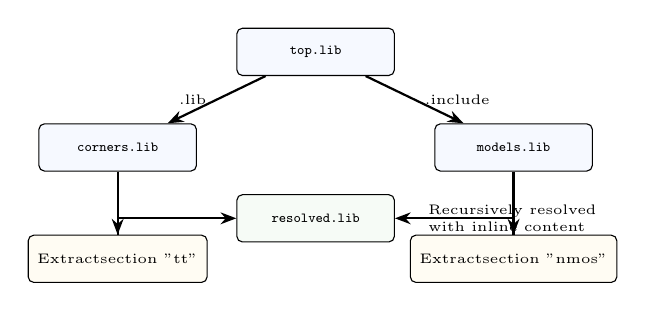
\begin{tikzpicture}[
    node distance=0.4cm,
    file/.style={rectangle, draw, rounded corners=2pt, fill=lightblue!40, minimum height=0.6cm, minimum width=2cm, font=\tiny\ttfamily},
    process/.style={rectangle, draw, rounded corners=2pt, fill=lightorange!40, minimum height=0.6cm, minimum width=1.5cm, font=\tiny},
    arrow/.style={-{Stealth[length=2mm]}, thick}
]

% Main file
\node[file] (main) {top.lib};

% Include directive
\node[file, below left=0.6cm and 0.5cm of main] (corner) {corners.lib};
\node[file, below right=0.6cm and 0.5cm of main] (models) {models.lib};

% Section extraction
\node[process, below=0.8cm of corner] (extract1) {Extract\\section "tt"};
\node[process, below=0.8cm of models] (extract2) {Extract\\section "nmos"};

% Result
\node[file, below=1.5cm of main, fill=lightgreen!40] (result) {resolved.lib};

% Arrows
\draw[arrow] (main) -- node[left, font=\tiny] {.lib} (corner);
\draw[arrow] (main) -- node[right, font=\tiny] {.include} (models);
\draw[arrow] (corner) -- (extract1);
\draw[arrow] (models) -- (extract2);
\draw[arrow] (extract1) |- (result);
\draw[arrow] (extract2) |- (result);

% Annotation
\node[right=0.3cm of result, font=\tiny, align=left] {Recursively resolved\\with inline content};

\end{tikzpicture}
\caption{OPTION G1: Include resolution workflow showing recursive section extraction from library files.}
\label{fig:include_resolve}
\end{figure}

\end{document}
